\documentclass{article}
\usepackage{graphicx}
\graphicspath{{res/}}
\usepackage{minted}

\title{Testando LaTex!}
\author{Kinan Principe}
\date{26 de Maio de 2078}

\begin{document}
\maketitle
\newpage
\tableofcontents
\newpage

\section{Introdução}

testando latex aqui agora!!
\begin{figure}[h]
    \centering
    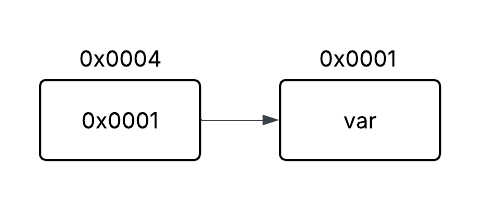
\includegraphics{ponteiro}
    \caption{Ponteiro como funciona...}
    \label{fig:ponteiro}
\end{figure}

\section{Listas}
\begin{itemize}
    \item apwoapodaw
    \item aaaaaaaaaaa
\end{itemize}

\begin{enumerate}
    \item apwoapodaw
    \item aaaaaaaaaaa
\end{enumerate}

\subsection{Código}

\begin{minted}{C}
for (int i = 0; i < 10; ++i) {
    printf("%d\n", i);
}
\end{minted}

\end{document}
